% Options for packages loaded elsewhere
\PassOptionsToPackage{unicode}{hyperref}
\PassOptionsToPackage{hyphens}{url}
%
\documentclass[
]{article}
\usepackage{amsmath,amssymb}
\usepackage{lmodern}
\usepackage{iftex}
\ifPDFTeX
  \usepackage[T1]{fontenc}
  \usepackage[utf8]{inputenc}
  \usepackage{textcomp} % provide euro and other symbols
\else % if luatex or xetex
  \usepackage{unicode-math}
  \defaultfontfeatures{Scale=MatchLowercase}
  \defaultfontfeatures[\rmfamily]{Ligatures=TeX,Scale=1}
\fi
% Use upquote if available, for straight quotes in verbatim environments
\IfFileExists{upquote.sty}{\usepackage{upquote}}{}
\IfFileExists{microtype.sty}{% use microtype if available
  \usepackage[]{microtype}
  \UseMicrotypeSet[protrusion]{basicmath} % disable protrusion for tt fonts
}{}
\makeatletter
\@ifundefined{KOMAClassName}{% if non-KOMA class
  \IfFileExists{parskip.sty}{%
    \usepackage{parskip}
  }{% else
    \setlength{\parindent}{0pt}
    \setlength{\parskip}{6pt plus 2pt minus 1pt}}
}{% if KOMA class
  \KOMAoptions{parskip=half}}
\makeatother
\usepackage{xcolor}
\usepackage[margin=1in]{geometry}
\usepackage{color}
\usepackage{fancyvrb}
\newcommand{\VerbBar}{|}
\newcommand{\VERB}{\Verb[commandchars=\\\{\}]}
\DefineVerbatimEnvironment{Highlighting}{Verbatim}{commandchars=\\\{\}}
% Add ',fontsize=\small' for more characters per line
\usepackage{framed}
\definecolor{shadecolor}{RGB}{248,248,248}
\newenvironment{Shaded}{\begin{snugshade}}{\end{snugshade}}
\newcommand{\AlertTok}[1]{\textcolor[rgb]{0.94,0.16,0.16}{#1}}
\newcommand{\AnnotationTok}[1]{\textcolor[rgb]{0.56,0.35,0.01}{\textbf{\textit{#1}}}}
\newcommand{\AttributeTok}[1]{\textcolor[rgb]{0.77,0.63,0.00}{#1}}
\newcommand{\BaseNTok}[1]{\textcolor[rgb]{0.00,0.00,0.81}{#1}}
\newcommand{\BuiltInTok}[1]{#1}
\newcommand{\CharTok}[1]{\textcolor[rgb]{0.31,0.60,0.02}{#1}}
\newcommand{\CommentTok}[1]{\textcolor[rgb]{0.56,0.35,0.01}{\textit{#1}}}
\newcommand{\CommentVarTok}[1]{\textcolor[rgb]{0.56,0.35,0.01}{\textbf{\textit{#1}}}}
\newcommand{\ConstantTok}[1]{\textcolor[rgb]{0.00,0.00,0.00}{#1}}
\newcommand{\ControlFlowTok}[1]{\textcolor[rgb]{0.13,0.29,0.53}{\textbf{#1}}}
\newcommand{\DataTypeTok}[1]{\textcolor[rgb]{0.13,0.29,0.53}{#1}}
\newcommand{\DecValTok}[1]{\textcolor[rgb]{0.00,0.00,0.81}{#1}}
\newcommand{\DocumentationTok}[1]{\textcolor[rgb]{0.56,0.35,0.01}{\textbf{\textit{#1}}}}
\newcommand{\ErrorTok}[1]{\textcolor[rgb]{0.64,0.00,0.00}{\textbf{#1}}}
\newcommand{\ExtensionTok}[1]{#1}
\newcommand{\FloatTok}[1]{\textcolor[rgb]{0.00,0.00,0.81}{#1}}
\newcommand{\FunctionTok}[1]{\textcolor[rgb]{0.00,0.00,0.00}{#1}}
\newcommand{\ImportTok}[1]{#1}
\newcommand{\InformationTok}[1]{\textcolor[rgb]{0.56,0.35,0.01}{\textbf{\textit{#1}}}}
\newcommand{\KeywordTok}[1]{\textcolor[rgb]{0.13,0.29,0.53}{\textbf{#1}}}
\newcommand{\NormalTok}[1]{#1}
\newcommand{\OperatorTok}[1]{\textcolor[rgb]{0.81,0.36,0.00}{\textbf{#1}}}
\newcommand{\OtherTok}[1]{\textcolor[rgb]{0.56,0.35,0.01}{#1}}
\newcommand{\PreprocessorTok}[1]{\textcolor[rgb]{0.56,0.35,0.01}{\textit{#1}}}
\newcommand{\RegionMarkerTok}[1]{#1}
\newcommand{\SpecialCharTok}[1]{\textcolor[rgb]{0.00,0.00,0.00}{#1}}
\newcommand{\SpecialStringTok}[1]{\textcolor[rgb]{0.31,0.60,0.02}{#1}}
\newcommand{\StringTok}[1]{\textcolor[rgb]{0.31,0.60,0.02}{#1}}
\newcommand{\VariableTok}[1]{\textcolor[rgb]{0.00,0.00,0.00}{#1}}
\newcommand{\VerbatimStringTok}[1]{\textcolor[rgb]{0.31,0.60,0.02}{#1}}
\newcommand{\WarningTok}[1]{\textcolor[rgb]{0.56,0.35,0.01}{\textbf{\textit{#1}}}}
\usepackage{graphicx}
\makeatletter
\def\maxwidth{\ifdim\Gin@nat@width>\linewidth\linewidth\else\Gin@nat@width\fi}
\def\maxheight{\ifdim\Gin@nat@height>\textheight\textheight\else\Gin@nat@height\fi}
\makeatother
% Scale images if necessary, so that they will not overflow the page
% margins by default, and it is still possible to overwrite the defaults
% using explicit options in \includegraphics[width, height, ...]{}
\setkeys{Gin}{width=\maxwidth,height=\maxheight,keepaspectratio}
% Set default figure placement to htbp
\makeatletter
\def\fps@figure{htbp}
\makeatother
\setlength{\emergencystretch}{3em} % prevent overfull lines
\providecommand{\tightlist}{%
  \setlength{\itemsep}{0pt}\setlength{\parskip}{0pt}}
\setcounter{secnumdepth}{-\maxdimen} % remove section numbering
\ifLuaTeX
  \usepackage{selnolig}  % disable illegal ligatures
\fi
\IfFileExists{bookmark.sty}{\usepackage{bookmark}}{\usepackage{hyperref}}
\IfFileExists{xurl.sty}{\usepackage{xurl}}{} % add URL line breaks if available
\urlstyle{same} % disable monospaced font for URLs
\hypersetup{
  pdftitle={Inference for categorical data},
  pdfauthor={Waheeb Algabri},
  hidelinks,
  pdfcreator={LaTeX via pandoc}}

\title{Inference for categorical data}
\author{Waheeb Algabri}
\date{}

\begin{document}
\maketitle

\hypertarget{getting-started}{%
\subsection{Getting Started}\label{getting-started}}

\hypertarget{load-packages}{%
\subsubsection{Load packages}\label{load-packages}}

In this lab, we will explore and visualize the data using the
\textbf{tidyverse} suite of packages, and perform statistical inference
using \textbf{infer}. The data can be found in the companion package for
OpenIntro resources, \textbf{openintro}.

Let's load the packages.

\begin{Shaded}
\begin{Highlighting}[]
\FunctionTok{library}\NormalTok{(tidyverse)}
\FunctionTok{library}\NormalTok{(openintro)}
\FunctionTok{library}\NormalTok{(infer)}
\FunctionTok{library}\NormalTok{(dplyr)}
\end{Highlighting}
\end{Shaded}

\hypertarget{the-data}{%
\subsubsection{The data}\label{the-data}}

You will be analyzing the same dataset as in the previous lab, where you
delved into a sample from the Youth Risk Behavior Surveillance System
(YRBSS) survey, which uses data from high schoolers to help discover
health patterns. The dataset is called \texttt{yrbss}.

First of all We will take a look at the columns of the data yrbss

\begin{Shaded}
\begin{Highlighting}[]
\FunctionTok{names}\NormalTok{(yrbss)}
\end{Highlighting}
\end{Shaded}

\begin{verbatim}
##  [1] "age"                      "gender"                  
##  [3] "grade"                    "hispanic"                
##  [5] "race"                     "height"                  
##  [7] "weight"                   "helmet_12m"              
##  [9] "text_while_driving_30d"   "physically_active_7d"    
## [11] "hours_tv_per_school_day"  "strength_training_7d"    
## [13] "school_night_hours_sleep"
\end{verbatim}

\begin{enumerate}
\def\labelenumi{\arabic{enumi}.}
\tightlist
\item
  What are the counts within each category for the amount of days these
  students have texted while driving within the past 30 days?
\end{enumerate}

\begin{Shaded}
\begin{Highlighting}[]
\NormalTok{yrbss }\SpecialCharTok{\%\textgreater{}\%}
  \FunctionTok{count}\NormalTok{(text\_while\_driving\_30d )}
\end{Highlighting}
\end{Shaded}

\begin{verbatim}
## # A tibble: 9 x 2
##   text_while_driving_30d     n
##   <chr>                  <int>
## 1 0                       4792
## 2 1-2                      925
## 3 10-19                    373
## 4 20-29                    298
## 5 3-5                      493
## 6 30                       827
## 7 6-9                      311
## 8 did not drive           4646
## 9 <NA>                     918
\end{verbatim}

We do a plot for it

\begin{Shaded}
\begin{Highlighting}[]
\NormalTok{plt\_data }\OtherTok{\textless{}{-}}\NormalTok{ yrbss }\SpecialCharTok{\%\textgreater{}\%} 
  \FunctionTok{count}\NormalTok{(text\_while\_driving\_30d)}

\FunctionTok{ggplot}\NormalTok{(}\AttributeTok{data=}\NormalTok{plt\_data, }\FunctionTok{aes}\NormalTok{(}\AttributeTok{x=}\NormalTok{text\_while\_driving\_30d, }\AttributeTok{y=}\NormalTok{n, }\AttributeTok{fill=}\FunctionTok{as.factor}\NormalTok{(text\_while\_driving\_30d))) }\SpecialCharTok{+}
  \FunctionTok{geom\_bar}\NormalTok{(}\AttributeTok{stat=}\StringTok{"identity"}\NormalTok{) }\SpecialCharTok{+} 
  \FunctionTok{labs}\NormalTok{(}
    \AttributeTok{x =} \StringTok{\textquotesingle{}How Many Days in the Past 30 Days Did You Text and Drive?\textquotesingle{}}\NormalTok{,}
    \AttributeTok{y =} \StringTok{\textquotesingle{}Number of Students\textquotesingle{}}\NormalTok{,}
    \AttributeTok{title =} \StringTok{\textquotesingle{}How Much Do Students Text and Drive?\textquotesingle{}}
\NormalTok{  ) }\SpecialCharTok{+} 
  \FunctionTok{coord\_flip}\NormalTok{()}
\end{Highlighting}
\end{Shaded}

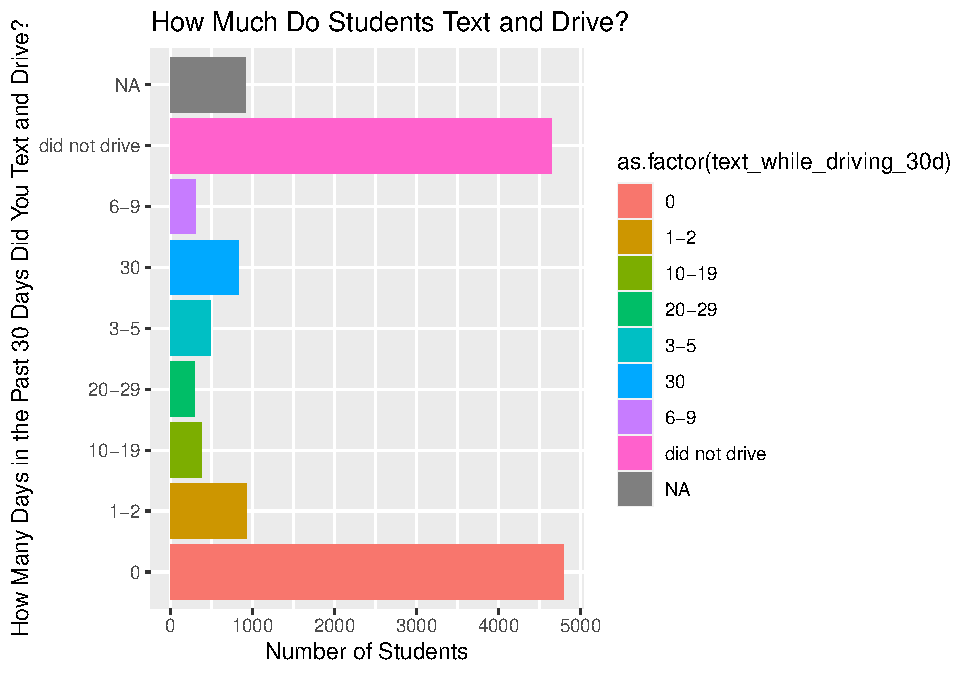
\includegraphics{Lab6_inf_for_categorical_data_files/figure-latex/unnamed-chunk-3-1.pdf}

\begin{enumerate}
\def\labelenumi{\arabic{enumi}.}
\setcounter{enumi}{1}
\tightlist
\item
  What is the proportion of people who have texted while driving every
  day in the past 30 days and never wear helmets?
\end{enumerate}

Remember that you can use \texttt{filter} to limit the dataset to just
non-helmet wearers. Here, we will name the dataset \texttt{no\_helmet}.

The ansswer will be

\begin{Shaded}
\begin{Highlighting}[]
\NormalTok{yrbss }\OtherTok{\textless{}{-}}\NormalTok{ yrbss }\SpecialCharTok{\%\textgreater{}\%} 
  \FunctionTok{mutate}\NormalTok{(}\AttributeTok{no\_helmet\_always\_texting =} 
           \FunctionTok{ifelse}\NormalTok{(text\_while\_driving\_30d }\SpecialCharTok{==} \StringTok{\textquotesingle{}30\textquotesingle{}} \SpecialCharTok{\&}
\NormalTok{                  helmet\_12m }\SpecialCharTok{==} \StringTok{\textquotesingle{}never\textquotesingle{}}\NormalTok{, }\ConstantTok{TRUE}\NormalTok{, }\ConstantTok{FALSE}\NormalTok{)) }

\NormalTok{yrbss }\SpecialCharTok{\%\textgreater{}\%} 
  \FunctionTok{filter}\NormalTok{(}\SpecialCharTok{!}\FunctionTok{is.na}\NormalTok{(no\_helmet\_always\_texting)) }\SpecialCharTok{\%\textgreater{}\%} 
    \FunctionTok{filter}\NormalTok{(no\_helmet\_always\_texting }\SpecialCharTok{==} \ConstantTok{TRUE}\NormalTok{) }\SpecialCharTok{\%\textgreater{}\%}
      \FunctionTok{nrow}\NormalTok{() }\SpecialCharTok{/} \FunctionTok{nrow}\NormalTok{(yrbss)}
\end{Highlighting}
\end{Shaded}

\begin{verbatim}
## [1] 0.03408673
\end{verbatim}

The code creates a new variable called
'no\_helmet\_always\_texting'which TRUE for people who have never worn
helmets and texted while driving every day in the past 30 days, and
FALSE otherwise.

\begin{center}\rule{0.5\linewidth}{0.5pt}\end{center}

\begin{Shaded}
\begin{Highlighting}[]
\FunctionTok{data}\NormalTok{(}\StringTok{\textquotesingle{}yrbss\textquotesingle{}}\NormalTok{, }\AttributeTok{package=}\StringTok{\textquotesingle{}openintro\textquotesingle{}}\NormalTok{)}
\NormalTok{no\_helmet }\OtherTok{\textless{}{-}}\NormalTok{ yrbss }\SpecialCharTok{\%\textgreater{}\%}
  \FunctionTok{filter}\NormalTok{(helmet\_12m }\SpecialCharTok{==} \StringTok{"never"}\NormalTok{)}
\end{Highlighting}
\end{Shaded}

Also, it may be easier to calculate the proportion if you create a new
variable that specifies whether the individual has texted every day
while driving over the past 30 days or not. We will call this variable
\texttt{text\_ind}.

\begin{Shaded}
\begin{Highlighting}[]
\NormalTok{no\_helmet }\OtherTok{\textless{}{-}}\NormalTok{ no\_helmet }\SpecialCharTok{\%\textgreater{}\%}
  \FunctionTok{mutate}\NormalTok{(}\AttributeTok{text\_ind =} \FunctionTok{ifelse}\NormalTok{(text\_while\_driving\_30d }\SpecialCharTok{==} \StringTok{"30"}\NormalTok{, }\StringTok{"yes"}\NormalTok{, }\StringTok{"no"}\NormalTok{))}
\end{Highlighting}
\end{Shaded}

\hypertarget{inference-on-proportions}{%
\subsection{Inference on proportions}\label{inference-on-proportions}}

When summarizing the YRBSS, the Centers for Disease Control and
Prevention seeks insight into the population \emph{parameters}. To do
this, you can answer the question, ``What proportion of people in your
sample reported that they have texted while driving each day for the
past 30 days?'' with a statistic; while the question ``What proportion
of people on earth have texted while driving each day for the past 30
days?'' is answered with an estimate of the parameter.

The inferential tools for estimating population proportion are analogous
to those used for means in the last chapter: the confidence interval and
the hypothesis test.

\begin{Shaded}
\begin{Highlighting}[]
\NormalTok{no\_helmet }\SpecialCharTok{\%\textgreater{}\%}
  \FunctionTok{specify}\NormalTok{(}\AttributeTok{response =}\NormalTok{ text\_ind, }\AttributeTok{success =} \StringTok{"yes"}\NormalTok{) }\SpecialCharTok{\%\textgreater{}\%}
  \FunctionTok{generate}\NormalTok{(}\AttributeTok{reps =} \DecValTok{1000}\NormalTok{, }\AttributeTok{type =} \StringTok{"bootstrap"}\NormalTok{) }\SpecialCharTok{\%\textgreater{}\%}
  \FunctionTok{prop\_test}\NormalTok{(text\_ind }\SpecialCharTok{\textasciitilde{}} \ConstantTok{NULL}\NormalTok{)}
\end{Highlighting}
\end{Shaded}

\begin{verbatim}
## # A tibble: 1 x 6
##   statistic chisq_df p_value alternative lower_ci upper_ci
##       <dbl>    <int>   <dbl> <chr>          <dbl>    <dbl>
## 1  4782706.        1       0 two.sided      0.929    0.929
\end{verbatim}

Note that since the goal is to construct an interval estimate for a
proportion, it's necessary to both include the \texttt{success} argument
within \texttt{specify}, which accounts for the proportion of non-helmet
wearers than have consistently texted while driving the past 30 days, in
this example, and that \texttt{stat} within \texttt{calculate} is here
``prop'', signaling that you are trying to do some sort of inference on
a proportion.

\begin{enumerate}
\def\labelenumi{\arabic{enumi}.}
\setcounter{enumi}{2}
\tightlist
\item
  What is the margin of error for the estimate of the proportion of
  non-helmet wearers that have texted while driving each day for the
  past 30 days based on this survey?
\end{enumerate}

\begin{Shaded}
\begin{Highlighting}[]
\NormalTok{ci }\OtherTok{\textless{}{-}}\NormalTok{ no\_helmet }\SpecialCharTok{\%\textgreater{}\%}
  \FunctionTok{specify}\NormalTok{(}\AttributeTok{response =}\NormalTok{ text\_ind, }\AttributeTok{success =} \StringTok{"yes"}\NormalTok{) }\SpecialCharTok{\%\textgreater{}\%}
  \FunctionTok{generate}\NormalTok{(}\AttributeTok{reps =} \DecValTok{1000}\NormalTok{, }\AttributeTok{type =} \StringTok{"bootstrap"}\NormalTok{) }\SpecialCharTok{\%\textgreater{}\%}
  \FunctionTok{calculate}\NormalTok{(}\AttributeTok{stat =} \StringTok{"prop"}\NormalTok{) }\SpecialCharTok{\%\textgreater{}\%}
  \FunctionTok{get\_ci}\NormalTok{(}\AttributeTok{level =} \FloatTok{0.95}\NormalTok{) }

\NormalTok{(ci}\SpecialCharTok{$}\NormalTok{upper\_ci }\SpecialCharTok{{-}}\NormalTok{ ci}\SpecialCharTok{$}\NormalTok{lower\_ci) }\SpecialCharTok{/} \DecValTok{2}
\end{Highlighting}
\end{Shaded}

I used this one which the professor modified.

\begin{Shaded}
\begin{Highlighting}[]
\NormalTok{ci}\OtherTok{\textless{}{-}}\NormalTok{ no\_helmet }\SpecialCharTok{\%\textgreater{}\%}
  \FunctionTok{specify}\NormalTok{(}\AttributeTok{response =}\NormalTok{ text\_ind, }\AttributeTok{success =} \StringTok{"yes"}\NormalTok{) }\SpecialCharTok{\%\textgreater{}\%}
  \FunctionTok{generate}\NormalTok{(}\AttributeTok{reps =} \DecValTok{1000}\NormalTok{, }\AttributeTok{type =} \StringTok{"bootstrap"}\NormalTok{) }\SpecialCharTok{\%\textgreater{}\%}
  \FunctionTok{prop\_test}\NormalTok{(text\_ind }\SpecialCharTok{\textasciitilde{}} \ConstantTok{NULL}\NormalTok{)}
\NormalTok{(ci}\SpecialCharTok{$}\NormalTok{upper\_ci }\SpecialCharTok{{-}}\NormalTok{ ci}\SpecialCharTok{$}\NormalTok{lower\_ci) }\SpecialCharTok{/} \DecValTok{2}
\end{Highlighting}
\end{Shaded}

\begin{verbatim}
## [1] 0.0001976564
\end{verbatim}

\begin{enumerate}
\def\labelenumi{\arabic{enumi}.}
\setcounter{enumi}{3}
\tightlist
\item
  Using the \texttt{infer} package, calculate confidence intervals for
  two other categorical variables (you'll need to decide which level to
  call ``success'', and report the associated margins of error. Interpet
  the interval in context of the data. It may be helpful to create new
  data sets for each of the two countries first, and then use these data
  sets to construct the confidence intervals.
\end{enumerate}

\begin{Shaded}
\begin{Highlighting}[]
\FunctionTok{names}\NormalTok{(yrbss)}
\end{Highlighting}
\end{Shaded}

\begin{verbatim}
##  [1] "age"                      "gender"                  
##  [3] "grade"                    "hispanic"                
##  [5] "race"                     "height"                  
##  [7] "weight"                   "helmet_12m"              
##  [9] "text_while_driving_30d"   "physically_active_7d"    
## [11] "hours_tv_per_school_day"  "strength_training_7d"    
## [13] "school_night_hours_sleep"
\end{verbatim}

\begin{Shaded}
\begin{Highlighting}[]
\NormalTok{yrbss }\SpecialCharTok{\%\textgreater{}\%}
  \FunctionTok{count}\NormalTok{(hours\_tv\_per\_school\_day, }\AttributeTok{sort=}\ConstantTok{TRUE}\NormalTok{)}
\end{Highlighting}
\end{Shaded}

\begin{verbatim}
## # A tibble: 8 x 2
##   hours_tv_per_school_day     n
##   <chr>                   <int>
## 1 2                        2705
## 2 <1                       2168
## 3 3                        2139
## 4 do not watch             1840
## 5 1                        1750
## 6 5+                       1595
## 7 4                        1048
## 8 <NA>                      338
\end{verbatim}

\begin{Shaded}
\begin{Highlighting}[]
\NormalTok{yrbss }\SpecialCharTok{\%\textgreater{}\%}
  \FunctionTok{count}\NormalTok{(school\_night\_hours\_sleep, }\AttributeTok{sort=}\ConstantTok{TRUE}\NormalTok{)}
\end{Highlighting}
\end{Shaded}

\begin{verbatim}
## # A tibble: 8 x 2
##   school_night_hours_sleep     n
##   <chr>                    <int>
## 1 7                         3461
## 2 8                         2692
## 3 6                         2658
## 4 5                         1480
## 5 <NA>                      1248
## 6 <5                         965
## 7 9                          763
## 8 10+                        316
\end{verbatim}

\hypertarget{watching-tv}{%
\subparagraph{Watching TV}\label{watching-tv}}

\begin{Shaded}
\begin{Highlighting}[]
\NormalTok{tv\_time}\OtherTok{\textless{}{-}}\NormalTok{ yrbss }\SpecialCharTok{\%\textgreater{}\%}
  \FunctionTok{filter}\NormalTok{(}\SpecialCharTok{!}\FunctionTok{is.na}\NormalTok{(hours\_tv\_per\_school\_day)) }\SpecialCharTok{\%\textgreater{}\%}
  \FunctionTok{mutate}\NormalTok{(}\AttributeTok{tv\_ind\_everyday =} \FunctionTok{ifelse}\NormalTok{(hours\_tv\_per\_school\_day }\SpecialCharTok{==} \StringTok{"\textless{}1"}\NormalTok{, }\StringTok{"yes"}\NormalTok{, }\StringTok{"no"}\NormalTok{))}

\NormalTok{tv\_time }\SpecialCharTok{\%\textgreater{}\%}
  \FunctionTok{count}\NormalTok{(tv\_ind\_everyday)}
\end{Highlighting}
\end{Shaded}

\begin{verbatim}
## # A tibble: 2 x 2
##   tv_ind_everyday     n
##   <chr>           <int>
## 1 no              11077
## 2 yes              2168
\end{verbatim}

13,245 students who reported their TV watching habits, 2,168 students
reported watching TV every day, while 11,077 students reported not
watching TV every day.

\begin{Shaded}
\begin{Highlighting}[]
\NormalTok{tv\_plot }\OtherTok{\textless{}{-}}\NormalTok{ tv\_time }\SpecialCharTok{\%\textgreater{}\%}
  \FunctionTok{count}\NormalTok{(tv\_ind\_everyday)}

\FunctionTok{ggplot}\NormalTok{(tv\_plot, }\FunctionTok{aes}\NormalTok{(}\AttributeTok{x =}\NormalTok{ tv\_ind\_everyday, }\AttributeTok{y =}\NormalTok{ n, }\AttributeTok{fill =}\NormalTok{ tv\_ind\_everyday)) }\SpecialCharTok{+}
  \FunctionTok{geom\_bar}\NormalTok{(}\AttributeTok{stat =} \StringTok{"identity"}\NormalTok{) }\SpecialCharTok{+}
  \FunctionTok{scale\_fill\_manual}\NormalTok{(}\AttributeTok{values =} \FunctionTok{c}\NormalTok{(}\StringTok{"yes"} \OtherTok{=} \StringTok{"skyblue"}\NormalTok{, }\StringTok{"no"} \OtherTok{=} \StringTok{"gray"}\NormalTok{)) }\SpecialCharTok{+}
  \FunctionTok{labs}\NormalTok{(}\AttributeTok{title =} \StringTok{"Proportion of Students Watching TV \textless{}1 Hour vs. 1+ Hour per School Day"}\NormalTok{,}
       \AttributeTok{x =} \StringTok{"TV Viewing Time"}\NormalTok{,}
       \AttributeTok{y =} \StringTok{"Count"}\NormalTok{) }\SpecialCharTok{+}
  \FunctionTok{theme\_minimal}\NormalTok{()}
\end{Highlighting}
\end{Shaded}

\includegraphics{Lab6_inf_for_categorical_data_files/figure-latex/unnamed-chunk-13-1.pdf}

\begin{Shaded}
\begin{Highlighting}[]
\NormalTok{tv\_time }\SpecialCharTok{\%\textgreater{}\%}
 \FunctionTok{specify}\NormalTok{(}\AttributeTok{response =}\NormalTok{ tv\_ind\_everyday, }\AttributeTok{success =} \StringTok{"yes"}\NormalTok{) }\SpecialCharTok{\%\textgreater{}\%}
 \FunctionTok{generate}\NormalTok{(}\AttributeTok{reps =} \DecValTok{1000}\NormalTok{, }\AttributeTok{type =} \StringTok{"bootstrap"}\NormalTok{) }\SpecialCharTok{\%\textgreater{}\%}
 \FunctionTok{calculate}\NormalTok{(}\AttributeTok{stat =} \StringTok{"prop"}\NormalTok{) }\SpecialCharTok{\%\textgreater{}\%}
 \FunctionTok{get\_ci}\NormalTok{(}\AttributeTok{level =} \FloatTok{0.95}\NormalTok{)}
\end{Highlighting}
\end{Shaded}

\begin{verbatim}
## # A tibble: 1 x 2
##   lower_ci upper_ci
##      <dbl>    <dbl>
## 1    0.158    0.170
\end{verbatim}

We are 95\% confident that the true proportion of students who watch TV
for less than 1 hour per school day and consider it as a ``yes''
response lies between 0.157 and 0.170.

\begin{Shaded}
\begin{Highlighting}[]
\FunctionTok{library}\NormalTok{(ggplot2)}

\NormalTok{tv\_time }\SpecialCharTok{\%\textgreater{}\%}
  \FunctionTok{count}\NormalTok{(tv\_ind\_everyday) }\SpecialCharTok{\%\textgreater{}\%}
  \FunctionTok{ggplot}\NormalTok{(}\FunctionTok{aes}\NormalTok{(}\AttributeTok{x =}\NormalTok{ tv\_ind\_everyday, }\AttributeTok{y =}\NormalTok{ n, }\AttributeTok{fill =}\NormalTok{ tv\_ind\_everyday)) }\SpecialCharTok{+}
  \FunctionTok{geom\_bar}\NormalTok{(}\AttributeTok{stat =} \StringTok{"identity"}\NormalTok{) }\SpecialCharTok{+}
  \FunctionTok{ggtitle}\NormalTok{(}\StringTok{"Proportion of Students Watching TV Less than 1 Hour per Day"}\NormalTok{) }\SpecialCharTok{+}
  \FunctionTok{xlab}\NormalTok{(}\StringTok{"Watch TV Less than 1 Hour per Day"}\NormalTok{) }\SpecialCharTok{+}
  \FunctionTok{ylab}\NormalTok{(}\StringTok{"Count of Students"}\NormalTok{) }\SpecialCharTok{+}
  \FunctionTok{scale\_fill\_manual}\NormalTok{(}\AttributeTok{values =} \FunctionTok{c}\NormalTok{(}\StringTok{"yes"} \OtherTok{=} \StringTok{"gray"}\NormalTok{, }\StringTok{"no"} \OtherTok{=} \StringTok{"skyblue"}\NormalTok{)) }\SpecialCharTok{+}
  \FunctionTok{theme}\NormalTok{(}\AttributeTok{plot.title =} \FunctionTok{element\_text}\NormalTok{(}\AttributeTok{hjust =} \FloatTok{0.5}\NormalTok{),}
        \AttributeTok{axis.text.x =} \FunctionTok{element\_text}\NormalTok{(}\AttributeTok{angle =} \DecValTok{0}\NormalTok{, }\AttributeTok{hjust =} \FloatTok{0.5}\NormalTok{))}
\end{Highlighting}
\end{Shaded}

\includegraphics{Lab6_inf_for_categorical_data_files/figure-latex/unnamed-chunk-15-1.pdf}

\hypertarget{sleeping-time}{%
\subparagraph{Sleeping time}\label{sleeping-time}}

\begin{Shaded}
\begin{Highlighting}[]
\NormalTok{sleep\_time}\OtherTok{\textless{}{-}}\NormalTok{ yrbss }\SpecialCharTok{\%\textgreater{}\%}
  \FunctionTok{filter}\NormalTok{(}\SpecialCharTok{!}\FunctionTok{is.na}\NormalTok{(school\_night\_hours\_sleep)) }\SpecialCharTok{\%\textgreater{}\%}
  \FunctionTok{mutate}\NormalTok{(}\AttributeTok{sleep\_ind\_everyday =} \FunctionTok{ifelse}\NormalTok{(school\_night\_hours\_sleep }\SpecialCharTok{==} \StringTok{"\textless{}5"}\NormalTok{, }\StringTok{"yes"}\NormalTok{, }\StringTok{"no"}\NormalTok{))}

\NormalTok{sleep\_time }\SpecialCharTok{\%\textgreater{}\%}
  \FunctionTok{count}\NormalTok{(sleep\_ind\_everyday)}
\end{Highlighting}
\end{Shaded}

\begin{verbatim}
## # A tibble: 2 x 2
##   sleep_ind_everyday     n
##   <chr>              <int>
## 1 no                 11370
## 2 yes                  965
\end{verbatim}

There are 965 students who reported getting less than 5 hours of sleep
on a typical school night, and there are 11,370 students who reported
getting 5 or more hours of sleep on a typical school night

\begin{Shaded}
\begin{Highlighting}[]
\FunctionTok{ggplot}\NormalTok{(}\AttributeTok{data =}\NormalTok{ sleep\_time, }\FunctionTok{aes}\NormalTok{(}\AttributeTok{x =}\NormalTok{ sleep\_ind\_everyday, }\AttributeTok{fill =}\NormalTok{ sleep\_ind\_everyday)) }\SpecialCharTok{+} 
  \FunctionTok{geom\_bar}\NormalTok{() }\SpecialCharTok{+} 
  \FunctionTok{scale\_fill\_manual}\NormalTok{(}\AttributeTok{values =} \FunctionTok{c}\NormalTok{(}\StringTok{"lightblue"}\NormalTok{, }\StringTok{"green"}\NormalTok{)) }\SpecialCharTok{+}
  \FunctionTok{labs}\NormalTok{(}\AttributeTok{x =} \StringTok{"Sleeping less than 5 hours on school nights"}\NormalTok{, }\AttributeTok{y =} \StringTok{"Count"}\NormalTok{) }\SpecialCharTok{+}
  \FunctionTok{theme\_minimal}\NormalTok{()}
\end{Highlighting}
\end{Shaded}

\includegraphics{Lab6_inf_for_categorical_data_files/figure-latex/unnamed-chunk-17-1.pdf}

\begin{Shaded}
\begin{Highlighting}[]
\NormalTok{sleep\_time }\SpecialCharTok{\%\textgreater{}\%}
 \FunctionTok{specify}\NormalTok{(}\AttributeTok{response =}\NormalTok{ sleep\_ind\_everyday, }\AttributeTok{success =} \StringTok{"yes"}\NormalTok{) }\SpecialCharTok{\%\textgreater{}\%}
 \FunctionTok{generate}\NormalTok{(}\AttributeTok{reps =} \DecValTok{1000}\NormalTok{, }\AttributeTok{type =} \StringTok{"bootstrap"}\NormalTok{) }\SpecialCharTok{\%\textgreater{}\%}
 \FunctionTok{calculate}\NormalTok{(}\AttributeTok{stat =} \StringTok{"prop"}\NormalTok{) }\SpecialCharTok{\%\textgreater{}\%}
 \FunctionTok{get\_ci}\NormalTok{(}\AttributeTok{level =} \FloatTok{0.95}\NormalTok{)}
\end{Highlighting}
\end{Shaded}

\begin{verbatim}
## # A tibble: 1 x 2
##   lower_ci upper_ci
##      <dbl>    <dbl>
## 1   0.0737   0.0831
\end{verbatim}

The confidence interval for the proportion of students who sleep less
than 5 hours per night on school days is (0.0739, 0.0828) with a 95\%
confidence level.it means that if we were to repeatedly sample from the
population and construct 95\% confidence intervals using the same method

\hypertarget{how-does-the-proportion-affect-the-margin-of-error}{%
\subsection{How does the proportion affect the margin of
error?}\label{how-does-the-proportion-affect-the-margin-of-error}}

Imagine you've set out to survey 1000 people on two questions: are you
at least 6-feet tall? and are you left-handed? Since both of these
sample proportions were calculated from the same sample size, they
should have the same margin of error, right? Wrong! While the margin of
error does change with sample size, it is also affected by the
proportion.

Think back to the formula for the standard error:
\(SE = \sqrt{p(1-p)/n}\). This is then used in the formula for the
margin of error for a 95\% confidence interval:

\[
ME = 1.96\times SE = 1.96\times\sqrt{p(1-p)/n} \,.
\] Since the population proportion \(p\) is in this \(ME\) formula, it
should make sense that the margin of error is in some way dependent on
the population proportion. We can visualize this relationship by
creating a plot of \(ME\) vs.~\(p\).

Since sample size is irrelevant to this discussion, let's just set it to
some value (\(n = 1000\)) and use this value in the following
calculations:

\begin{Shaded}
\begin{Highlighting}[]
\NormalTok{n }\OtherTok{\textless{}{-}} \DecValTok{1000}
\end{Highlighting}
\end{Shaded}

The first step is to make a variable \texttt{p} that is a sequence from
0 to 1 with each number incremented by 0.01. You can then create a
variable of the margin of error (\texttt{me}) associated with each of
these values of \texttt{p} using the familiar approximate formula
(\(ME = 2 \times SE\)).

\begin{Shaded}
\begin{Highlighting}[]
\NormalTok{p }\OtherTok{\textless{}{-}} \FunctionTok{seq}\NormalTok{(}\AttributeTok{from =} \DecValTok{0}\NormalTok{, }\AttributeTok{to =} \DecValTok{1}\NormalTok{, }\AttributeTok{by =} \FloatTok{0.01}\NormalTok{)}
\NormalTok{me }\OtherTok{\textless{}{-}} \DecValTok{2} \SpecialCharTok{*} \FunctionTok{sqrt}\NormalTok{(p }\SpecialCharTok{*}\NormalTok{ (}\DecValTok{1} \SpecialCharTok{{-}}\NormalTok{ p)}\SpecialCharTok{/}\NormalTok{n)}
\end{Highlighting}
\end{Shaded}

Lastly, you can plot the two variables against each other to reveal
their relationship. To do so, we need to first put these variables in a
data frame that you can call in the \texttt{ggplot} function.

\begin{Shaded}
\begin{Highlighting}[]
\NormalTok{dd }\OtherTok{\textless{}{-}} \FunctionTok{data.frame}\NormalTok{(}\AttributeTok{p =}\NormalTok{ p, }\AttributeTok{me =}\NormalTok{ me)}
\FunctionTok{ggplot}\NormalTok{(}\AttributeTok{data =}\NormalTok{ dd, }\FunctionTok{aes}\NormalTok{(}\AttributeTok{x =}\NormalTok{ p, }\AttributeTok{y =}\NormalTok{ me)) }\SpecialCharTok{+} 
  \FunctionTok{geom\_line}\NormalTok{() }\SpecialCharTok{+}
  \FunctionTok{labs}\NormalTok{(}\AttributeTok{x =} \StringTok{"Population Proportion"}\NormalTok{, }\AttributeTok{y =} \StringTok{"Margin of Error"}\NormalTok{)}
\end{Highlighting}
\end{Shaded}

\includegraphics{Lab6_inf_for_categorical_data_files/figure-latex/me-plot-1.pdf}

\begin{enumerate}
\def\labelenumi{\arabic{enumi}.}
\setcounter{enumi}{4}
\tightlist
\item
  Describe the relationship between \texttt{p} and \texttt{me}. Include
  the margin of error vs.~population proportion plot you constructed in
  your answer. For a given sample size, for which value of \texttt{p} is
  margin of error maximized?
\end{enumerate}

The relationship between `p' and `ME' is non-linear and parabolic. As p
moves away from 0.5 in either direction, the margin of error increases.
This makes sense since the maximum margin of error occurs when the
proportion is closest to 0.5, which is the point of greatest
uncertainty. When p is either very close to 0 or 1, there is less
uncertainty since the sample proportion is close to the true population
proportion. The plot of ME vs.~p shows that the margin of error reaches
its maximum value of around 0.032 at p = 0.5 for a sample size of 1000.

\hypertarget{success-failure-condition}{%
\subsection{Success-failure condition}\label{success-failure-condition}}

We have emphasized that you must always check conditions before making
inference. For inference on proportions, the sample proportion can be
assumed to be nearly normal if it is based upon a random sample of
independent observations and if both \(np \geq 10\) and
\(n(1 - p) \geq 10\). This rule of thumb is easy enough to follow, but
it makes you wonder: what's so special about the number 10?

The short answer is: nothing. You could argue that you would be fine
with 9 or that you really should be using 11. What is the ``best'' value
for such a rule of thumb is, at least to some degree, arbitrary.
However, when \(np\) and \(n(1-p)\) reaches 10 the sampling distribution
is sufficiently normal to use confidence intervals and hypothesis tests
that are based on that approximation.

You can investigate the interplay between \(n\) and \(p\) and the shape
of the sampling distribution by using simulations. Play around with the
following app to investigate how the shape, center, and spread of the
distribution of \(\hat{p}\) changes as \(n\) and \(p\) changes.

\begin{enumerate}
\def\labelenumi{\arabic{enumi}.}
\setcounter{enumi}{5}
\tightlist
\item
  Describe the sampling distribution of sample proportions at
  \(n = 300\) and \(p = 0.1\). Be sure to note the center, spread, and
  shape.
\end{enumerate}

At \(n=300\) and \(p=0.1\), the sampling distribution of sample
proportions is centered around \(0.1\) and has a \textbf{spread} of
approximately \(0.03\). \textbf{The shape} of the distribution is
approximately normal, although there is some skewness towards the right
due to the low value of \(p\). The distribution is unimodal and
symmetric for the most part, although there is a slight bump on the
right side of the distribution due to the skewness. Overall, the
sampling distribution of sample proportions at these values of \(n\) and
\(p\) satisfies the success-failure condition with \(np=30\) and
\(n(1-p)=270\), so we \textbf{can use the normal approximation to make
inferences about the population proportion based on the sample
proportion.}

\begin{Shaded}
\begin{Highlighting}[]
\FunctionTok{library}\NormalTok{(ggplot2)}

\NormalTok{pp }\OtherTok{\textless{}{-}} \FunctionTok{data.frame}\NormalTok{(}\AttributeTok{p\_hat =} \FunctionTok{rep}\NormalTok{(}\DecValTok{0}\NormalTok{, }\DecValTok{5000}\NormalTok{))}
\ControlFlowTok{for}\NormalTok{(i }\ControlFlowTok{in} \DecValTok{1}\SpecialCharTok{:}\DecValTok{5000}\NormalTok{)\{}
\NormalTok{  samp }\OtherTok{\textless{}{-}} \FunctionTok{sample}\NormalTok{(}\FunctionTok{c}\NormalTok{(}\ConstantTok{TRUE}\NormalTok{, }\ConstantTok{FALSE}\NormalTok{), }\DecValTok{300}\NormalTok{, }\AttributeTok{replace =} \ConstantTok{TRUE}\NormalTok{, }\AttributeTok{prob =} \FunctionTok{c}\NormalTok{(}\FloatTok{0.1}\NormalTok{, }\FloatTok{0.9}\NormalTok{))}
\NormalTok{  pp}\SpecialCharTok{$}\NormalTok{p\_hat[i] }\OtherTok{\textless{}{-}} \FunctionTok{sum}\NormalTok{(samp }\SpecialCharTok{==} \ConstantTok{TRUE}\NormalTok{) }\SpecialCharTok{/} \DecValTok{300}
\NormalTok{\}}

\FunctionTok{ggplot}\NormalTok{(}\AttributeTok{data =}\NormalTok{ pp, }\FunctionTok{aes}\NormalTok{(}\AttributeTok{x =}\NormalTok{ p\_hat)) }\SpecialCharTok{+}
  \FunctionTok{geom\_histogram}\NormalTok{(}\AttributeTok{binwidth =} \FloatTok{0.025}\NormalTok{, }\AttributeTok{color =} \StringTok{"black"}\NormalTok{, }\AttributeTok{fill =} \StringTok{"white"}\NormalTok{) }\SpecialCharTok{+}
  \FunctionTok{labs}\NormalTok{(}\AttributeTok{title =} \StringTok{"Sampling Distribution of Sample Proportions at n=300 and p=0.1"}\NormalTok{,}
       \AttributeTok{x =} \StringTok{"Sample Proportion"}\NormalTok{, }\AttributeTok{y =} \StringTok{"Count"}\NormalTok{) }\SpecialCharTok{+}
  \FunctionTok{theme\_minimal}\NormalTok{()}
\end{Highlighting}
\end{Shaded}

\includegraphics{Lab6_inf_for_categorical_data_files/figure-latex/unnamed-chunk-19-1.pdf}

\begin{enumerate}
\def\labelenumi{\arabic{enumi}.}
\setcounter{enumi}{6}
\tightlist
\item
  Keep \(n\) constant and change \(p\). How does the shape, center, and
  spread of the sampling distribution vary as \(p\) changes. You might
  want to adjust min and max for the \(x\)-axis for a better view of the
  distribution.
\end{enumerate}

\begin{Shaded}
\begin{Highlighting}[]
\FunctionTok{library}\NormalTok{(ggplot2)}

\NormalTok{pp }\OtherTok{\textless{}{-}} \FunctionTok{data.frame}\NormalTok{(}\AttributeTok{p\_hat =} \FunctionTok{rep}\NormalTok{(}\DecValTok{0}\NormalTok{, }\DecValTok{5000}\NormalTok{))}
\ControlFlowTok{for}\NormalTok{(i }\ControlFlowTok{in} \DecValTok{1}\SpecialCharTok{:}\DecValTok{5000}\NormalTok{)\{}
\NormalTok{  samp }\OtherTok{\textless{}{-}} \FunctionTok{sample}\NormalTok{(}\FunctionTok{c}\NormalTok{(}\ConstantTok{TRUE}\NormalTok{, }\ConstantTok{FALSE}\NormalTok{), }\DecValTok{300}\NormalTok{, }\AttributeTok{replace =} \ConstantTok{TRUE}\NormalTok{, }\AttributeTok{prob =} \FunctionTok{c}\NormalTok{(}\FloatTok{0.1}\NormalTok{, }\FloatTok{0.9}\NormalTok{))}
\NormalTok{  pp}\SpecialCharTok{$}\NormalTok{p\_hat[i] }\OtherTok{\textless{}{-}} \FunctionTok{sum}\NormalTok{(samp }\SpecialCharTok{==} \ConstantTok{TRUE}\NormalTok{) }\SpecialCharTok{/} \DecValTok{300}
\NormalTok{\}}

\NormalTok{bw }\OtherTok{\textless{}{-}} \FunctionTok{diff}\NormalTok{(}\FunctionTok{range}\NormalTok{(pp}\SpecialCharTok{$}\NormalTok{p\_hat)) }\SpecialCharTok{/} \DecValTok{30}

\FunctionTok{ggplot}\NormalTok{(}\AttributeTok{data =}\NormalTok{ pp, }\FunctionTok{aes}\NormalTok{(}\AttributeTok{x =}\NormalTok{ p\_hat)) }\SpecialCharTok{+}
  \FunctionTok{geom\_histogram}\NormalTok{(}\AttributeTok{binwidth =}\NormalTok{ bw) }\SpecialCharTok{+}
  \FunctionTok{xlim}\NormalTok{(}\DecValTok{0}\NormalTok{, }\FloatTok{0.5}\NormalTok{) }\SpecialCharTok{+}
  \FunctionTok{ggtitle}\NormalTok{(}\StringTok{"Sampling distribution of sample proportions at n=300 and varying p"}\NormalTok{)}
\end{Highlighting}
\end{Shaded}

\includegraphics{Lab6_inf_for_categorical_data_files/figure-latex/unnamed-chunk-20-1.pdf}

As we can see from the plot, when p is closer to 0.5, the center of the
sampling distribution is closer to p itself. The spread of the
distribution remains approximately the same regardless of the value of
p.~The shape of the distribution starts off skewed to the right when p
is very small, becomes more symmetric as p increases, and becomes skewed
to the left when p is very large.

\begin{enumerate}
\def\labelenumi{\arabic{enumi}.}
\setcounter{enumi}{7}
\tightlist
\item
  Now also change \(n\). How does \(n\) appear to affect the
  distribution of \(\hat{p}\)?
\end{enumerate}

\begin{Shaded}
\begin{Highlighting}[]
\FunctionTok{set.seed}\NormalTok{(}\DecValTok{123}\NormalTok{)}
\NormalTok{n\_values }\OtherTok{\textless{}{-}} \FunctionTok{c}\NormalTok{(}\DecValTok{30}\NormalTok{, }\DecValTok{100}\NormalTok{, }\DecValTok{300}\NormalTok{, }\DecValTok{1000}\NormalTok{)}
\NormalTok{p }\OtherTok{\textless{}{-}} \FloatTok{0.3}

\NormalTok{results }\OtherTok{\textless{}{-}} \FunctionTok{tibble}\NormalTok{()}

\ControlFlowTok{for}\NormalTok{(n }\ControlFlowTok{in}\NormalTok{ n\_values)\{}
\NormalTok{  p\_hat }\OtherTok{\textless{}{-}} \FunctionTok{replicate}\NormalTok{(}\DecValTok{10000}\NormalTok{, }\FunctionTok{mean}\NormalTok{(}\FunctionTok{sample}\NormalTok{(}\FunctionTok{c}\NormalTok{(}\DecValTok{0}\NormalTok{,}\DecValTok{1}\NormalTok{), n, }\AttributeTok{replace =} \ConstantTok{TRUE}\NormalTok{, }\AttributeTok{prob =} \FunctionTok{c}\NormalTok{(}\DecValTok{1}\SpecialCharTok{{-}}\NormalTok{p, p))))}
\NormalTok{  results }\OtherTok{\textless{}{-}}\NormalTok{ results }\SpecialCharTok{\%\textgreater{}\%} 
    \FunctionTok{bind\_rows}\NormalTok{(}\FunctionTok{tibble}\NormalTok{(}\AttributeTok{n =}\NormalTok{ n, }\AttributeTok{p\_hat =}\NormalTok{ p\_hat))}
\NormalTok{\}}

\FunctionTok{ggplot}\NormalTok{(results, }\FunctionTok{aes}\NormalTok{(}\AttributeTok{x=}\NormalTok{p\_hat, }\AttributeTok{fill=}\FunctionTok{factor}\NormalTok{(n))) }\SpecialCharTok{+} 
  \FunctionTok{geom\_histogram}\NormalTok{(}\AttributeTok{binwidth=}\FloatTok{0.02}\NormalTok{, }\AttributeTok{position=}\StringTok{"identity"}\NormalTok{, }\AttributeTok{alpha=}\FloatTok{0.5}\NormalTok{) }\SpecialCharTok{+}
  \FunctionTok{scale\_fill\_discrete}\NormalTok{(}\AttributeTok{name=}\StringTok{"Sample size (n)"}\NormalTok{) }\SpecialCharTok{+} 
  \FunctionTok{ggtitle}\NormalTok{(}\FunctionTok{paste0}\NormalTok{(}\StringTok{"Sampling distribution of p̂ at different sample sizes with p = "}\NormalTok{, p)) }\SpecialCharTok{+}
  \FunctionTok{xlab}\NormalTok{(}\StringTok{"Sample proportion (p̂)"}\NormalTok{) }\SpecialCharTok{+} \FunctionTok{ylab}\NormalTok{(}\StringTok{"Count"}\NormalTok{)}
\end{Highlighting}
\end{Shaded}

\includegraphics{Lab6_inf_for_categorical_data_files/figure-latex/unnamed-chunk-21-1.pdf}

As we increase the sample size, the center of the sampling distribution
of \(\hat{p}\) remains the same as the true population proportion, but
the spread decreases. This means that as we increase \(n\), we are more
likely to get an estimate of \(\hat{p}\) that is closer to the true
population proportion \(p\).

\begin{center}\rule{0.5\linewidth}{0.5pt}\end{center}

\hypertarget{more-practice}{%
\subsection{More Practice}\label{more-practice}}

For some of the exercises below, you will conduct inference comparing
two proportions. In such cases, you have a response variable that is
categorical, and an explanatory variable that is also categorical, and
you are comparing the proportions of success of the response variable
across the levels of the explanatory variable. This means that when
using \texttt{infer}, you need to include both variables within
\texttt{specify}.

\begin{enumerate}
\def\labelenumi{\arabic{enumi}.}
\setcounter{enumi}{8}
\tightlist
\item
  Is there convincing evidence that those who sleep 10+ hours per day
  are more likely to strength train every day of the week? As always,
  write out the hypotheses for any tests you conduct and outline the
  status of the conditions for inference. If you find a significant
  difference, also quantify this difference with a confidence interval.
\end{enumerate}

Let p1 denote the proportion of students who sleep 10 or more hours per
day and strength train every day of the week. Let p2 denote the
proportion of all other students who strength train every day of the
week. The null hypothesis is that there is no difference in the
proportions of students who strength train every day of the week between
those who sleep 10+ hours per day and all other students. The
alternative hypothesis is that there is a difference in proportions
between the two groups. This can be written as:

\(Ho: p1 - p2 = 0\)

\(HA: p1 - p2 ≠ 0\)

A hypothesis test is conducted using 95\% confidence intervals (α =
0.05) on bootstrap samples of the test statistic (p1 - p2).

\begin{Shaded}
\begin{Highlighting}[]
\NormalTok{yrbss }\SpecialCharTok{\%\textgreater{}\%}
  \FunctionTok{mutate}\NormalTok{(}
    \AttributeTok{very\_sleepy =} \FunctionTok{ifelse}\NormalTok{(school\_night\_hours\_sleep }\SpecialCharTok{==} \StringTok{\textquotesingle{}10+\textquotesingle{}}\NormalTok{, }\ConstantTok{TRUE}\NormalTok{, }\ConstantTok{FALSE}\NormalTok{),}
    \AttributeTok{bodybuilder =} \FunctionTok{ifelse}\NormalTok{(strength\_training\_7d }\SpecialCharTok{==} \StringTok{\textquotesingle{}7\textquotesingle{}}\NormalTok{, }\ConstantTok{TRUE}\NormalTok{, }\ConstantTok{FALSE}\NormalTok{)       }
\NormalTok{  ) }\SpecialCharTok{\%\textgreater{}\%}
  \FunctionTok{filter}\NormalTok{(}\SpecialCharTok{!}\FunctionTok{is.na}\NormalTok{(very\_sleepy) }\SpecialCharTok{\&} \SpecialCharTok{!}\FunctionTok{is.na}\NormalTok{(bodybuilder)) }\SpecialCharTok{\%\textgreater{}\%}
    \FunctionTok{specify}\NormalTok{(bodybuilder }\SpecialCharTok{\textasciitilde{}}\NormalTok{ very\_sleepy, }\AttributeTok{success =} \StringTok{\textquotesingle{}TRUE\textquotesingle{}}\NormalTok{) }\SpecialCharTok{\%\textgreater{}\%}
    \FunctionTok{generate}\NormalTok{(}\AttributeTok{reps =} \DecValTok{1000}\NormalTok{, }\AttributeTok{type =} \StringTok{"bootstrap"}\NormalTok{) }\SpecialCharTok{\%\textgreater{}\%}
    \FunctionTok{calculate}\NormalTok{(}\AttributeTok{stat =} \StringTok{"diff in props"}\NormalTok{, }\AttributeTok{order =} \FunctionTok{c}\NormalTok{(}\StringTok{\textquotesingle{}FALSE\textquotesingle{}}\NormalTok{, }\StringTok{\textquotesingle{}TRUE\textquotesingle{}}\NormalTok{)) }\SpecialCharTok{\%\textgreater{}\%}
    \FunctionTok{get\_ci}\NormalTok{(}\AttributeTok{level =} \FloatTok{0.95}\NormalTok{)}
\end{Highlighting}
\end{Shaded}

\begin{verbatim}
## # A tibble: 1 x 2
##   lower_ci upper_ci
##      <dbl>    <dbl>
## 1   -0.157  -0.0533
\end{verbatim}

The lower\_ci value (-0.157) represents the lower bound of the
confidence interval, which suggests that the true difference in
proportions between the two groups may be as low as -0.157. Similarly,
the upper\_ci value (-0.0584) represents the upper bound of the
confidence interval, which suggests that the true difference in
proportions may be as high as -0.0584.

Since the confidence interval does not contain the value of zero, we can
conclude that there is a statistically significant difference between
the proportions of students who sleep 10+ hours per day and strength
train every day of the week and those who do not. This means that those
who sleep 10+ hours per day are either more or less likely to strength
train every day of the week compared to all other students.

The confidence interval calculated from the bootstrap samples of the
difference in proportions between the two groups is {[}-0.157,
-0.0584{]}. Since this interval does not contain zero, we can reject the
null hypothesis that p1 - p2 = 0 at the 0.05 level of significance.

Since the difference in proportions is negative and the confidence
interval does not include zero, we can conclude that the proportion of
students who sleep 10+ hours per day and strength train every day of the
week (p1) is significantly lower than the proportion of all other
students who strength train every day of the week (p2) at the 0.05 level
of significance. Therefore, we can say that p1 \textless{} p2.

\begin{Shaded}
\begin{Highlighting}[]
\FunctionTok{library}\NormalTok{(ggplot2)}

\NormalTok{yrbss }\SpecialCharTok{\%\textgreater{}\%}
  \FunctionTok{mutate}\NormalTok{(}
    \AttributeTok{very\_sleepy =} \FunctionTok{ifelse}\NormalTok{(school\_night\_hours\_sleep }\SpecialCharTok{==} \StringTok{\textquotesingle{}10+\textquotesingle{}}\NormalTok{, }\ConstantTok{TRUE}\NormalTok{, }\ConstantTok{FALSE}\NormalTok{),}
    \AttributeTok{bodybuilder =} \FunctionTok{ifelse}\NormalTok{(strength\_training\_7d }\SpecialCharTok{==} \StringTok{\textquotesingle{}7\textquotesingle{}}\NormalTok{, }\ConstantTok{TRUE}\NormalTok{, }\ConstantTok{FALSE}\NormalTok{)}
\NormalTok{  ) }\SpecialCharTok{\%\textgreater{}\%}
  \FunctionTok{filter}\NormalTok{(}\SpecialCharTok{!}\FunctionTok{is.na}\NormalTok{(very\_sleepy) }\SpecialCharTok{\&} \SpecialCharTok{!}\FunctionTok{is.na}\NormalTok{(bodybuilder)) }\SpecialCharTok{\%\textgreater{}\%}
  \FunctionTok{group\_by}\NormalTok{(very\_sleepy) }\SpecialCharTok{\%\textgreater{}\%}
  \FunctionTok{summarize}\NormalTok{(}\AttributeTok{prop\_bodybuilder =} \FunctionTok{mean}\NormalTok{(bodybuilder)) }\SpecialCharTok{\%\textgreater{}\%}
  \FunctionTok{ggplot}\NormalTok{(}\FunctionTok{aes}\NormalTok{(}\AttributeTok{x =}\NormalTok{ very\_sleepy, }\AttributeTok{y =}\NormalTok{ prop\_bodybuilder)) }\SpecialCharTok{+}
  \FunctionTok{geom\_col}\NormalTok{() }\SpecialCharTok{+}
  \FunctionTok{ggtitle}\NormalTok{(}\StringTok{"Proportion of Students who Strength Train Daily"}\NormalTok{) }\SpecialCharTok{+}
  \FunctionTok{xlab}\NormalTok{(}\StringTok{"Sleep Hours per Night"}\NormalTok{) }\SpecialCharTok{+}
  \FunctionTok{ylab}\NormalTok{(}\StringTok{"Proportion"}\NormalTok{) }\SpecialCharTok{+}
  \FunctionTok{ylim}\NormalTok{(}\DecValTok{0}\NormalTok{, }\FloatTok{0.5}\NormalTok{) }\SpecialCharTok{+}
  \FunctionTok{theme\_bw}\NormalTok{()}
\end{Highlighting}
\end{Shaded}

\includegraphics{Lab6_inf_for_categorical_data_files/figure-latex/unnamed-chunk-23-1.pdf}

\begin{enumerate}
\def\labelenumi{\arabic{enumi}.}
\setcounter{enumi}{9}
\tightlist
\item
  Let's say there has been no difference in likeliness to strength train
  every day of the week for those who sleep 10+ hours. What is the
  probablity that you could detect a change (at a significance level of
  0.05) simply by chance? \emph{Hint:} Review the definition of the Type
  1 error.
\end{enumerate}

Assuming that there is no actual difference in the proportion of those
who strength train every day of the week for those who sleep 10+ hours,
the probability of observing a significant difference purely by chance
(Type 1 error) can be calculated as the significance level, which is
0.05 in this case.

\begin{enumerate}
\def\labelenumi{\arabic{enumi}.}
\setcounter{enumi}{10}
\tightlist
\item
  Suppose you're hired by the local government to estimate the
  proportion of residents that attend a religious service on a weekly
  basis. According to the guidelines, the estimate must have a margin of
  error no greater than 1\% with 95\% confidence. You have no idea what
  to expect for \(p\). How many people would you have to sample to
  ensure that you are within the guidelines?\\
  \emph{Hint:} Refer to your plot of the relationship between \(p\) and
  margin of error. This question does not require using a dataset.
\end{enumerate}

To ensure that the margin of error is no greater than 1\% with 95\%
confidence, we need to find the sample size required for a given p such
that the margin of error is less than or equal to 1\%.

From the plot of the relationship between p and margin of error, we can
see that the margin of error is highest when p = 0.5. Therefore, to be
conservative, we will assume that p = 0.5, which gives us the largest
possible sample size required.

The formula for calculating the sample size is:

\(n = (z*σ / E)^2\)

where z is the z-score corresponding to the desired level of confidence
\((z = 1.96 for 95% confidence)
\), \(σ\)is the standard deviation of the population (which we don't
know, so we'll use the worst-case scenario of p=0.5), and E is the
maximum allowable margin of error (0.01).

Substituting these values, we get:

\(n = (1.96 * sqrt(0.5 * 0.5) / 0.01)^2\)

\(n = 9604\)

Therefore, we would need to sample at least 9604 residents to ensure
that our estimate of the proportion of residents that attend a religious
service on a weekly basis has a margin of error no greater than 1\% with
95\% confidence, assuming the worst-case scenario of p=0.5.

\begin{Shaded}
\begin{Highlighting}[]
\CommentTok{\# Create a function to calculate margin of error}
\NormalTok{margin\_of\_error }\OtherTok{\textless{}{-}} \ControlFlowTok{function}\NormalTok{(p\_hat, n) \{}
\NormalTok{  z\_star }\OtherTok{\textless{}{-}} \FunctionTok{qnorm}\NormalTok{(}\FloatTok{0.975}\NormalTok{)}
  \FunctionTok{sqrt}\NormalTok{(p\_hat}\SpecialCharTok{*}\NormalTok{(}\DecValTok{1}\SpecialCharTok{{-}}\NormalTok{p\_hat)}\SpecialCharTok{/}\NormalTok{n) }\SpecialCharTok{*}\NormalTok{ z\_star}
\NormalTok{\}}

\CommentTok{\# Create a sequence of sample proportions from 0 to 1 with increment of 0.01}
\NormalTok{p\_hat\_seq }\OtherTok{\textless{}{-}} \FunctionTok{seq}\NormalTok{(}\DecValTok{0}\NormalTok{, }\DecValTok{1}\NormalTok{, }\AttributeTok{by =} \FloatTok{0.01}\NormalTok{)}

\CommentTok{\# Calculate margin of error for each sample proportion}
\NormalTok{margin\_of\_error\_seq }\OtherTok{\textless{}{-}} \FunctionTok{margin\_of\_error}\NormalTok{(p\_hat\_seq, }\DecValTok{1000}\NormalTok{)}

\CommentTok{\# Combine the two vectors into a data frame}
\NormalTok{data }\OtherTok{\textless{}{-}} \FunctionTok{data.frame}\NormalTok{(}\AttributeTok{p\_hat =}\NormalTok{ p\_hat\_seq, }\AttributeTok{margin\_of\_error =}\NormalTok{ margin\_of\_error\_seq)}

\CommentTok{\# Create the plot}
\FunctionTok{ggplot}\NormalTok{(data, }\FunctionTok{aes}\NormalTok{(}\AttributeTok{x =}\NormalTok{ p\_hat, }\AttributeTok{y =}\NormalTok{ margin\_of\_error)) }\SpecialCharTok{+} 
  \FunctionTok{geom\_line}\NormalTok{() }\SpecialCharTok{+}
  \FunctionTok{scale\_x\_continuous}\NormalTok{(}\StringTok{"Sample Proportion"}\NormalTok{) }\SpecialCharTok{+}
  \FunctionTok{scale\_y\_continuous}\NormalTok{(}\StringTok{"Margin of Error"}\NormalTok{, }\AttributeTok{limits =} \FunctionTok{c}\NormalTok{(}\DecValTok{0}\NormalTok{, }\FloatTok{0.02}\NormalTok{)) }\SpecialCharTok{+}
  \FunctionTok{geom\_hline}\NormalTok{(}\AttributeTok{yintercept =} \FloatTok{0.01}\NormalTok{, }\AttributeTok{linetype =} \StringTok{"dashed"}\NormalTok{) }\SpecialCharTok{+}
  \FunctionTok{annotate}\NormalTok{(}\StringTok{"text"}\NormalTok{, }\AttributeTok{x =} \FloatTok{0.5}\NormalTok{, }\AttributeTok{y =} \FloatTok{0.015}\NormalTok{, }\AttributeTok{label =} \StringTok{"Max Margin of Error = 1\%"}\NormalTok{, }\AttributeTok{size =} \DecValTok{4}\NormalTok{, }\AttributeTok{color =} \StringTok{"red"}\NormalTok{) }\SpecialCharTok{+}
  \FunctionTok{theme\_bw}\NormalTok{()}
\end{Highlighting}
\end{Shaded}

\includegraphics{Lab6_inf_for_categorical_data_files/figure-latex/unnamed-chunk-24-1.pdf}

The plot shows a curve that reaches its peak at p\_hat = 0.5, which
means that the margin of error is largest when the sample proportion is
around 0.5. As the sample proportion gets closer to 0 or 1, the margin
of error gets smaller. The dashed line represents the maximum margin of
error of 1\% that we need to achieve, and the red text shows the label
for that line. Based on this plot, we can see that we would need a
sample size of around 10,000 to achieve a margin of error no greater
than 1\% with 95\% confidence. * * *

\end{document}
